% GitHub cvitanov/reducesymm/tingnan/3gener.tex

% Predrag                                       2014-04-18
	
\chapter{3 generator tiling}
\label{c-3gener}

% \item[2014-07-14 Predrag]
My intuition is that the symbolic dynamics is robust under varying
the disk spacing $w$ - for sufficiently large $w$ there is no pruning, and all
of our short/long hop orbits are allowed. As $w$ decreases, some of them get pruned,
but symbolic dynamics should not change - if you label disks, it labels the same
sequence of disk visitations (I do not how to prove this, so I might be wrong.)

\refFig{fig:cycle026A} is a nice illustration; there are
many equivalent sequences of three generators $\{s,\ell,f\}$ and
the problem is that of determining isomorphisms between deterministic
finite automata. Here we show how to `quotient' equivalent
substrings.

We know that on the elementary
cell level there are only 11 (or 12 -  one isomorphism) symbols, so maybe
we can figure how to uniquely relabel the $\{s,\ell,f\}$ itineraries in
terms of such set.


%%%%%%%%%%%%%%\item[Figure ?]%%%%%%%%%%%%%%%%%%%%%%%%%%%%%%%%%%%%%%%%%%
\begin{figure}
\begin{center}
(a) 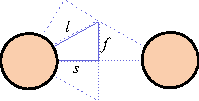
\includegraphics[width=0.45\textwidth]{7diskFundDflips}
(b) 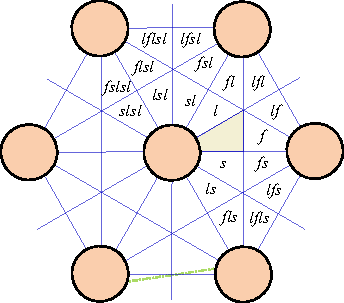
\includegraphics[width=0.45\textwidth]{7diskFundDtiles}
\end{center}
\caption{
(a) The three generators of tiling of the plane by a fundamental domain:
two generators of \Dn{12} tiling, reflection $s$ across the short
disk-disk separation, reflection  $\ell$  across the long disk-disk
separation;
and
a translation generator $f$ that pivots (`flips') a disk center to disk
center by flip across the symmetry line normal to the short disk-disk
separation.
(5) Tiling of the 7-disk by copies of the fundamental domain, labelled
by a (not unique) sequence of the three generators
$\{s,\ell,f\}$, chosen so that each sequence contain one and only on
    disk-to-disk pivot $f$.
        }
\label{7diskFundDflipsA}
\end{figure}
%%%%%%%%%%%%%%\item[Figure 4]%%%%%%%%%%%%%%%%%%%%%%%%%%%%%%%%%%%%%%%%%%

% \item[2014-06-02, 2014-06-08 Predrag]
\refFig{7diskFundDflipsA}\,(a) illustrates the three generators
\beq
    \{s,\ell,f\}
\,.
\ee{c-3gener}
In the international
crystallographic notation, our hexagonal lattice is called $p6mm$,
with point group $6mm$,
where
prefix $p$ indicates that the unit cell is primitive (not centered),
\beq
\Group = \{
e, C_6^+, C_6^-, C_3^+, C_3^-, C_2,
\sigma_{d1}, \sigma_{d2}, \sigma_{d3},
\sigma_{v1},\sigma_{v2}, \sigma_{v3}
\}
\,,
\ee{D12generatorsA}
with $s=\sigma_{d}$ the reflection across the
short disk-disk separation, and $\ell=\sigma_{v}$ reflection across the
long disk-disk separation generators of \Dn{12}. The entire space group
is then generated by adding a disk-to-disk generator $f$ that pivots a
disk center to disk center by flip across the symmetry line normal to the
short disk-disk separation.
We find it convenient to define $C$ as the generator of cyclic rotations
by $\pi/3$,
\[
\ell s = C_6^- = C
\,,\quad
C^6 = e
\,;\qquad
s \ell =  C_6^+
\,,\qquad
s  =  C_6^+ \ell
\,.
\]
There are two short paths from disk to disk: $f$, which keeps the sense
of orientation, and $sf=fs$ which changes it.

\begin{figure}
\includegraphics[width=\textwidth]{7diskFUndDtilesEquiv}
\caption{Shortest equivalent sequences.}
\label{fig:symbolEquivA}
\end{figure}


The (hopefully complete) list of the
equivalence relations, \ie, different sequences of operations reaching
the same copy of the fundamental domain is:
\beq
s s = e
\,,\quad
\ell \ell = e
\,,\quad
f f = e
\,,\quad
C^6 = e
\,;\qquad
f s = s f
\,,\quad
f \ell f=\ell f \ell
\,.
\ee{3generEquiv}
The two flips $f s = s f$ act at $90^0$ and hence commute.
As shown in \reffig{fig:symbolEquivA}, $f\ell f$ and $\ell f \ell$
map the fundamental domain to the same copy. Finally, $C^6 = e$ ensures
that the tiling is hexagonal.

Our task is to generate all distinct
itineraries from $\{s,\ell,f\}$, by pre-pending a letter to a given sequence.
Repeats of the 3 letters are not allowed (so tree of admissible sequences
is binary), and neither is the sixth repeat of the
rotation $C$. The remaining two equivalence relations we impose by
crossing out any itinerary that contains block $f s$ or block $f\ell f$.
Prohibition of the block $f s$ implies that $s$ is always followed by $\ell$,
\ie, we can replace the $s$ at last position in an itinerary by
$ s \to \ell s = C$,
with $\ell C$ prohibited in the next step.
We start with the three starting letters $\{s,\ell,f\}$, and generate the admissible
itineraries tree as follows:
\bea
&s & \quad\quad \ell \quad\qquad f
    \continue
& C & \quad s \ell, f \ell \qquad s f , \ell f
    \continue
&s C, f C & \quad
    C \ell; s f \ell , \ell f \ell \qquad
        C f ; s \ell f
    \label{3generTree}\\
&C^2; s f C, \ell f C & \quad
    s C \ell, f C \ell; C f \ell ;  s \ell f \ell  \qquad
       s C f, f C f  ; C \ell f
    \continue
&s C^2, f C^2; C f C, s \ell f C  & \quad
    C^2 \ell; s f C \ell , \ell f C \ell ;
            s C f \ell , f C f \ell ;  C \ell f \ell  \qquad
       C^2 f ;  s f C f ,  \ell f C f  ; s C \ell f , f C \ell f
\nnu
\eea
All longer equivalence relations in \reffig{fig:symbolEquivA}
can be reduced to the above primitive ones:
\[
f s \ell = s f \ell
\,,\qquad
      f \ell s \ell f \ell f s
    = f C \ell \ell f C
    = (f C)^2
\]

Treat every itinerary as a cycle, simplify by using cyclic permutations:
\bea
&\cycle{s} & \cycle{\ell} \quad \cycle{f} ;
 \quad \cycle{s \ell} \quad \cycle{s f} \quad \cycle{\ell f} ;
 \quad    \cycle{s \ell f} ;
 \quad  \cycle{s \ell f \ell} ;
 \quad  \cycle{s \ell s   f \ell}
\,.
    \label{3generCycl}
\eea

Is $\cycle{f}$ allowed??? Tingnan is right, need to mark the billiard wall as well?

Here is a list (incomplete) of the fundamental domain fixed points, \ie,
sequences containing at least one $f$ obtained by cyclic repeats of
itineraries in \refeq{3generTree} (see \reffig{7diskFundDflipsA}\,(b)):
\bea
\cycle{f} &=& \cycle{06} \,,\qquad \mbox{shift} = 0
    \continue
\cycle{fs} &=&  \cycle{08} =  \cycle{26} \,,\qquad
\mbox{shift} = \jEigvec[0]-\jEigvec[2]
    \continue
\cycle{f\ell} &=&  \cycle{048} \,,\qquad \mbox{shift} = 0
    \continue
\cycle{f\ell s} &=& \cycle{24}
 \,,\qquad \mbox{shift} = 2\jEigvec[0]-\jEigvec[2]
    \continue
\cycle{f\ell s\ell} &=& \cycle{0\underline{10}8642}
 \,,\qquad \mbox{shift} = 0
    \continue
 \cycle{f s\ell s\ell} &=&  \cycle{???}
 \,,\qquad \mbox{shift} = ?
\,.
\eea
In other words, the 6 fundamental domain symbols are 3 rotations
$\{e,C_6,C_6^2\}$ together with 3 rotations followed by a reflection.

Cycles $\cycle{\ell f\ell}$,
$\cycle{\ell fs\ell}$,
\etc, are not distinct fixed points, because using cyclic symmetry and
$\ell^2 =1$ we have
 $\cycle{\ell f\ell}=\cycle{f}$,
$\cycle{\ell fs\ell}=\cycle{fs}$, \etc.


For practice, let's work out a
few  cycles composed of short flights only.
\refFig{7diskFundDflips2}: conversion of elementary cell \po s $\to$
fundamental domain fixed points for the short 2-cycle, 3-cycle and
6-cycle.
Adding long \po s and \rpo s should result in 11 fundamental domain fixed
points in all, and the 11 letters of alphabet of \refref{LorentzDiff}.

%%%%%%%%%%%%%%\item[Figure ?]%%%%%%%%%%%%%%%%%%%%%%%%%%%%%%%%%%%%%%%%%%
\begin{figure}
\begin{center}
(a)\includegraphics[width=0.43\textwidth]{7diskFundDflips2}
(b)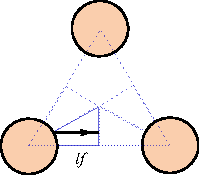
\includegraphics[width=0.43\textwidth]{7diskFundDflips3}
\\
(c)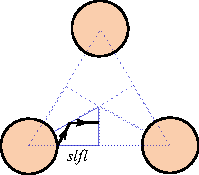
\includegraphics[width=0.43\textwidth]{7diskFundDflips6}
\end{center}
\caption{
(a) Elementary cell short 2-cycle , with multiplicity 3 corresponds to
the fixed pint $f$ in fundamental domain, $\cycle{02}=\cycle{f^2}$;
(b) Elementary cell short clockwise 3-cycle $\cycle{084}$, and
counterclockwise 3-cycle $\cycle{048}$, in
fundamental domain $\cycle{048}=\cycle{(\ell f)^3}$.
(c) Elementary cell short 6-cycle of multiplicity 2, in
fundamental domain $\cycle{0\underline{10}8642}=\cycle{(s\ell f\ell )^6}$.
    }
\label{7diskFundDflips2A}
\end{figure}
%%%%%%%%%%%%%%\item[Figure 4]%%%%%%%%%%%%%%%%%%%%%%%%%%%%%%%%%%%%%%%%%%

This is no new the 2-cycle:
$ \cycle{s \ell f \ell f \ell}
= \cycle{s f \ell f f \ell}
= \cycle{s f}
\neq \cycle{046\underline{10}}$,

There is also 2-cycle $\cycle{0369}$ (once we start including longs).

\begin{figure}
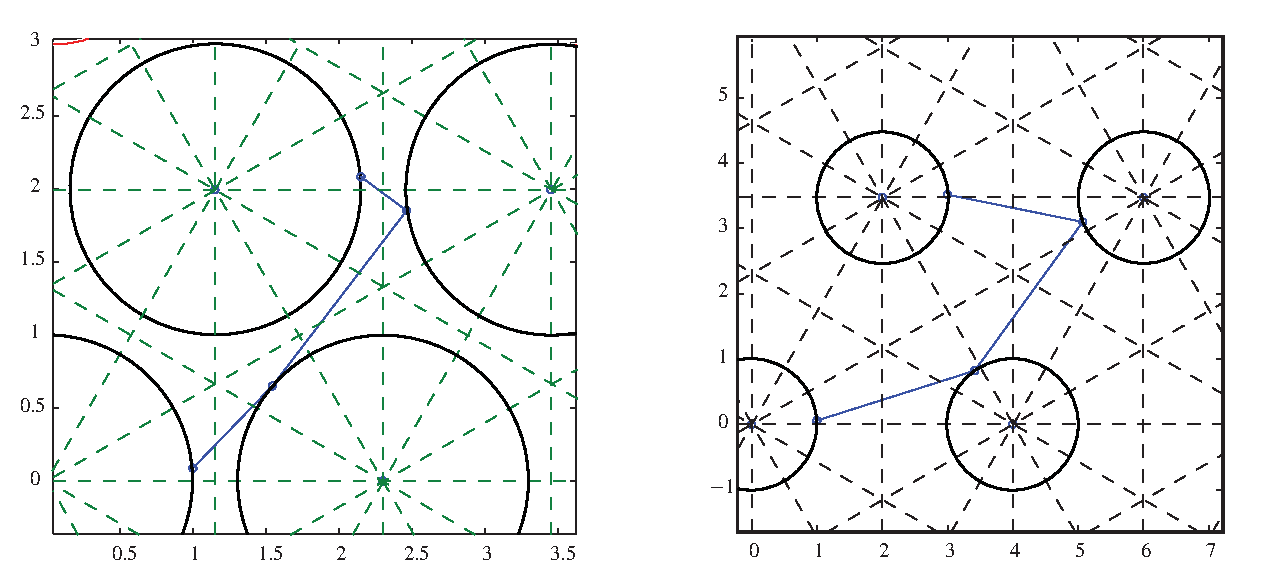
\includegraphics[width=\textwidth]{cycle026.pdf}
\caption{3-cycle \cycle{026} for $w=0.3$ (left) and $w=2$ (right). }
\label{fig:cycle026A}
\end{figure}

% \item[2014-07-11 Tingnan]
I have checked a few cycles and their new symbolic representations. For
example, $\cycle{026}$ and \cycle{0260628}. For cycle $\cycle{026}$ and
$w=0.3$, \reffig{fig:cycle026A}\,(left panel),
the symbolic sequence is $\cycle{f\ell sf\ell f fs}$.
% \item[2014-07-14 Predrag]
Using $f f = 1$
\[
\cycle{f\ell sf\ell f fs}
    = \cycle{f\ell sf\ell s}
    = \cycle{f\ell s}
\,.
\]
For $w=2.0$, \reffig{fig:cycle026A}\,(right panel), the
sequence is slightly different, $f\ell s\ell f \ell fs$, but with the
equivalence relations
% $f \ell f=\ell f \ell$
% \item[2014-07-14 Predrag]
% You are sure that $f\ell f$ equals $\ell f \ell$?
% The have different numbers of flips.
$f s = s f$ and $f \ell f = \ell f \ell$ the end sequence is the
same,
\[
\cycle{f\ell s\ell f \ell fs}
    = \cycle{\ell s\ell f \ell s}
    = \cycle{\ell s f \ell f s}
    = \cycle{\ell s f}
\,.
\]

% \item[2014-07-11 Tingnan]
Similar results can be obtained for $\cycle{0260628}$ in
\reffig{fig:cycle0260628A}.
\[
\cycle{f \ell f s f \ell ...}
\,.
\]
(2014-07-14 Predrag: I give up, let computer do this...)
I have also
checked a few cases when long flights are involved, and the same
conclusion holds: the symbolic sequence we proposed is invariant to
parameter changes.

\begin{figure}
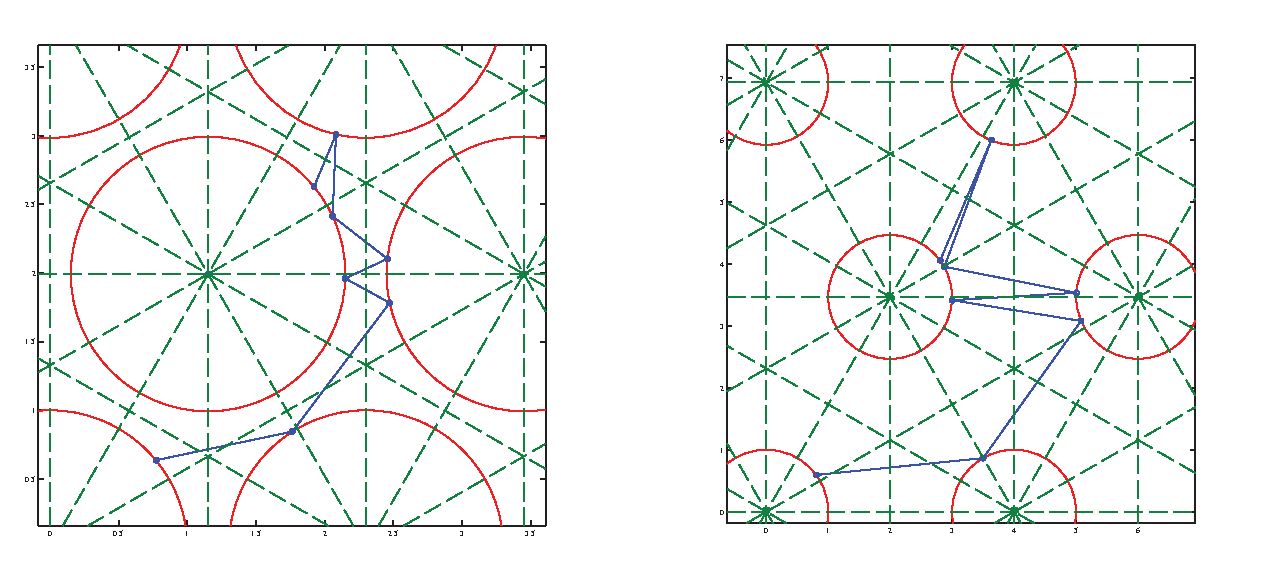
\includegraphics[width=\textwidth]{cycle0260628}
\caption{\label{fig:cycle0260628A}
7-cycle \cycle{0260628} for $w=0.3$ (left) and $w=2$ (right).
}
\end{figure}

\begin{table}
\begin{center}
\begin{tabular}{r}
Symbols and itinerary \\\hline
$\ell$  \\
$s\ell$ \\
$\ell s \ell$ \\
$s \ell s \ell$ \\
$\ell s \ell s \ell$ \\
$s\ell s \ell s \ell$ \\
$s$  \\
$\ell s$ \\
$s \ell s $ \\
$\ell s \ell s$ \\
$s \ell s \ell s$ \\
- \\\hline
\end{tabular}
\end{center}
\caption{All 11 combinations without flip $f$. }
\label{tab:11slcombos}
\end{table}
(2014-07-17 Tingnan) Obervation: since the free flight cannot cross over a disk, the sequence $sl$ or $ls$ can at most appear 3 times, and the $C^6=e$ relation can be re-written as $(s\ell)^3=(\ell s)^3$ (i.e. rotating 180 degree either clockwise or counter clockwise would give the same tile). This also reduces the number of symbols in the state machine(Fig.~\ref{fig:statemachine}). Following the graph, We can generate at most 11 strings without flip $f$(Table ~\ref{tab:11slcombos}). For a single flip, $f$ can be sandwiched by 
any two of the combinations (including the $-$ as a place holder). A valid (and longer) sequence can be generated according to the graph.
\begin{figure}
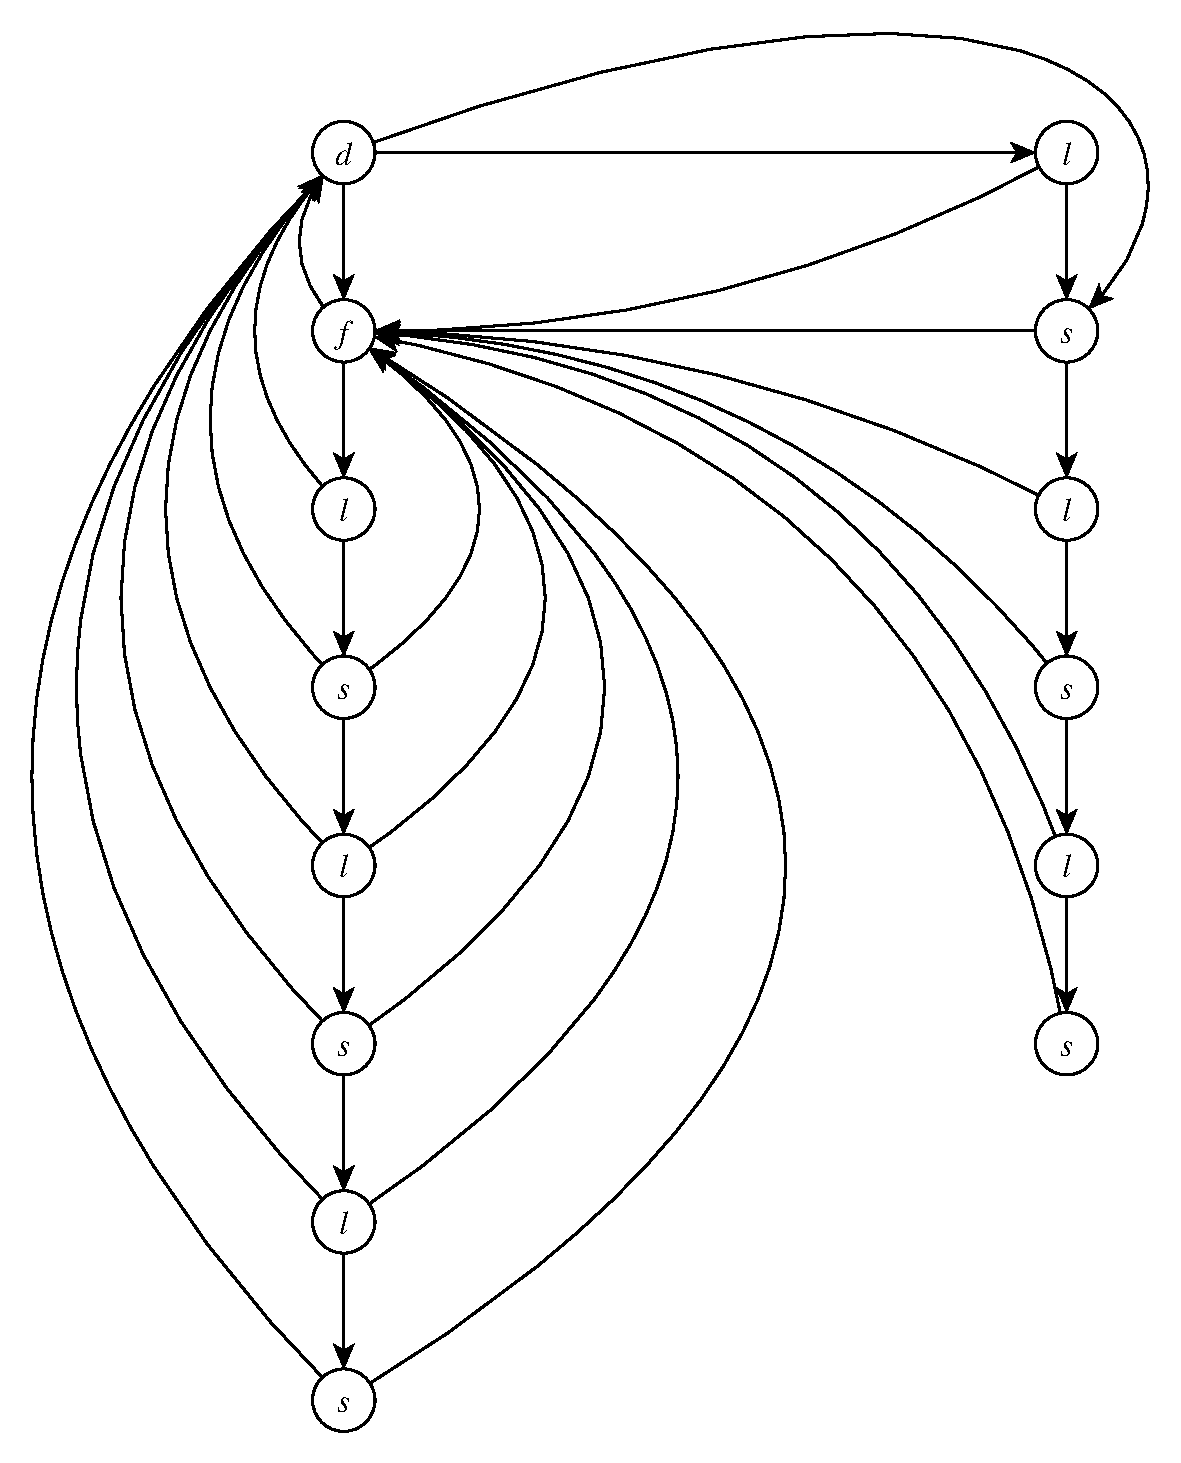
\includegraphics[width=\textwidth]{statemachine.pdf}
\caption{\label{fig:statemachine} The Markov graph for the symbols.
}
\end{figure}